\section{RESEARCH METHODOLOGY} \normalfont 
\label{sec:method}

This section describes the overarching research methodology, the methods used and how they were applied, a methodological reflection, and a discussion of other methodologies that were considered, and which are as valid for this thesis. 

%  Further, the nature of the thesis and the RQs require a mixed-method approach using both qualitative and quantitative methods.

To explore game design as a Human-AI collaborative task, how game content might be generated and adapted, and how to better integrate AI in these systems and processes, this thesis mainly follows a ~\acrfull{dsrm}~\cite{DSRM-Hevner}.~\acrshort{dsrm} aims at producing innovative artifacts to address a set of problems, challenges, and research questions within an area of concern. This thesis investigates this through a mix of qualitative and quantitative methods. Qualitative methods such as user studies, interviews, and controlled experiments, to collect data from usability, experience, and clarity of the interaction. Quantitative methods such as simulation and experimentation, where the goal is to evaluate specific properties, trade-offs, and the scope of the artifacts. 

Moreover, artifacts created for the purpose of creating technology-innovation, are categorized according to~\acrshort{dsrm} in the following four types: \emph{constructs}, \emph{models}, \emph{methods}, and \emph{instantiations}. \emph{Constructs} are the symbols and composed language to represent and define the problem and possible solutions. \emph{Models} are the representations of the problems and solutions, which uses the previously defined constructs. \emph{Methods} are the processes that are followed to solve the represented problem. Finally, \emph{instantiations} are the final systems used to demonstrate that the other categories can be used as solutions to address the defined problems~\cite{DSRM-Hevner}. Through the thesis, four artifacts have been developed.

% The first one relates more to the definition of \textbf{instantiation}

\subsection{Evolutionary Dungeon Designer}

the~\acrlong{edd}, defined as \textbf{instantiation}, is the main research tool in this thesis where we can investigate game design and multiple content creation aspects as well as the interaction between human designer and computational designer.~\acrshort{edd} has enough flexibility to explore this interaction and to use it as a research tool to investigate the performance, behavior, and usability of multiple AI techniques and models. Thus, by developing and evaluating~\acrshort{edd}, it is possible to support the development and creative expression of humans, and to test systems that aim at improving and exploring the co-creative, co-creation, and co-design capabilities of~\acrshort{micc}.

We have developed four systems that build on top of~\acrshort{edd} to explore this interaction.~\acrshort{edd} main content generation area is within level design, which is explored and developed in \textsc{papers i-iii, v, vi}. Within~\acrshort{edd}, we have also explored the generation of narrative, and its connection and usability alongside the level design facet. Narrative is explored and implemented in QuestGram (\textsc{paper vii}), TropeTwist (\textsc{paper x}), and Story Designer (\textsc{paper xi}).

% These four systems 

\subsection{Computational Designer}

The computational designer (composed of multiple AI techniques) related to \textbf{model, method, and instantiation}, where each underlying AI technique is implemented, used, and evaluated within~\acrshort{edd}. Through this, it is explored how different approaches affect the human-AI interaction, while aiming towards fostering creativity, reducing workload, and creating a much tighter Human-AI dynamic. These AI techniques range from addressing specific challenges such as explicit controllability by human designers and their aesthetic consideration (\textsc{paper ii}), to the use of quality-diversity algorithms to generate content in different facets (\textsc{papers iii, v, x, xi}), to the use of different type of grammars such as L-systems (\textsc{paper viii}) and graph grammars (\textsc{paper x}).

Furthermore, it is relevant to explore not only what algorithms and AI techniques are used for the Computational Designer, but also its role in the interaction. Thus, the role of the computational designer and its agency was preliminary explored in \textsc{paper xii}. We analyzed and evaluated through a controlled experiment in the form of user study, the interaction and user experience of the human designer when the computational designer gains more agency in the final design. 

\subsection{Temporal Expressive Range Analysis}

%\begin{itemize}
%    \item Explain briefly ERA
%    \item Explain TERA and how it can be used. Why was it proposed? what was missing that needed it?
%    \item Paper I present this and when/where I used 
%\end{itemize}

Expressive Range Analysis (ERA) is a popular and relevant method to evaluate content generators, since it allows the inspection of the diversity and expressiveness of a content generator with regards to feature dimensions and use as a comparison with other algorithms~\cite{shaker_procedural_2016,cook_danesh_2016,horn_comparative_2014}. In \textsc{paper viii}, we extended ERA and presented Temporal Expressive Range Analysis (TERA) as a method to better use ERAs in interactive PCG and MI-CC systems. TERA relates in DSRM as a \textbf{method}, and is proposed as a evaluation method to analyze and assess theses interactive systems. TERAs allow the inspection and analysis of changes in the ERA over a defined period such as generations, design editions, or time; and how the algorithms react and adapt to constant changes in the input. We introduced an aggregated and non-aggregated version. Non-aggregated TERAs show the delta maps of the generator, meaning where the generator has focused and the space covered for a specific period part. Aggregated TERAs show the density of generated content over all the defined period and the coverage up to the specific period. TERAs were used in \textsc{papers viii and xi} to assess the content generated with the IC MAP-Elites for game levels and narrative structures. 

%as presented in the background (), is a common and relevant method to evaluate content generator, especially in PCG, since it allows the inspection of the diversity of a content generator with regards to feature dimensions. 

%The following cases examine TERAs following the different scenarios presented in figure~\ref{figs:roomsexperiments}. Different cases will use either an aggregated TERA step by step or a non-aggregated version showing each step's specific scores in the evaluated dimensions. Each figure's caption and respective case will indicate what type of TERA is used. Non-Aggregated TERAs show the delta maps in the search, meaning where the search has focused and the space covered for a specific step. On the other hand, aggregated TERAs show the density of generated individuals over all steps and the coverage up to the specific step. In each TERA, we also show as an orange dot where the current design is in relation to the used and tested dimensions. Case 1 and 2 examine aggregated TERAs, while case 3 examines non-agreggated TERAs.

%Therefore, the contributions of this paper are two-fold. On the one hand, we present Temporal Expressive Range Analysis (TERA) as a novel way to analyze interactive PCG. TERAs allow us to inspect and analyze the changes in the expressive range over a defined period, which in our case, are design editions. On the other hand, using TERAs, we explored and analyzed how population dynamics react and adapt to constant changes in the IC MAP-Elites for level generation of 2D adventure games.

\subsection{Designer Personas}

In this thesis, we argue about the importance of \emph{Designer Modeling} in MI-CC systems as a step towards adaptability, tailor-made experiences, and better interactions. We approached and investigated this in \textsc{papers iv and ix}. Nevertheless, in \textsc{paper ix} we presented and proposed an approach, related in DSRM as a \textbf{method}, for a data-driven modeling of the design process, style, and goals. This method allows for the identification of \emph{Designer Personas} as archetypical paths through a clustered design style space in the respective design space. \emph{Designer Personas} take the task of recognizing style and adapting content towards that to a higher abstraction layer, where both the final design and individual design edits are less relevant, and the process and trajectory through a clustered style space based on designer's data is highlighted.  For instance, rooms for a game like the binding of Isaac~\cite{mcmillen_binding_2011} could be classified based on multiple characteristics such as the room's objectives regarding enemies and treasures, access to different areas, or hidden encounter and treasures. Moreover, different designers could reach the same room style through different paths, where the focus along the creation could vary. Some designers would focus on the room's architecture before anything else, whereas others would focus first on the objectives a player must achieve.

%In this thesis, we argue about the importance of \emph{Designer Modeling} in MI-CC systems as a step towards adaptability, tailor-made experiences, and better interactions. We approached and investigated this in \textsc{paper v, x, and xiv} and as part of this kappa's contribution. Nevertheless, in \textsc{paper x} we presented and proposed an approach, related in DSRM as a \textbf{method}, for a data-driven modeling of the design process, style, and goals. This method allows for the identification of \emph{Designer Personas} as archetypical paths through a clustered design style space in the respective design space. \emph{Designer Personas} take the task of recognizing style and adapting content towards that to a higher abstraction layer, where both the final design and individual design edits are less relevant, and the process and trajectory through a clustered style space based on designer's data is highlighted.  For instance, rooms for a game like the binding of Isaac~\cite{mcmillen_binding_2011} could be classified based on multiple characteristics such as the room's objectives regarding enemies and treasures, access to different areas, or hidden encounter and treasures. Moreover, different designers could reach the same room style through different paths, where the focus along the creation could vary. Some designers would focus on the room's architecture before anything else, whereas others would focus first on the objectives a player must achieve.

%where individual design edits are less relevant ... is not only an alternative method for designer modeling, but it can be used not 

%An alternative method could be to identify a set of styles that most designers follow when creating content, and model how the designer traverse such a style space. For instance, rooms for a game like the binding of Isaac~\cite{mcmillen_binding_2011} could be classified based on multiple characteristics such as the room's objectives regarding enemies and treasures, access to different areas, or hidden encounter and treasures. Moreover, different designers could reach the same room style through different paths, where the focus along the creation could vary. Some designers would focus on the room's architecture before anything else, whereas others would focus first on the objectives a player must achieve. These designer models could then be combined with search-based~\cite{Togelius2011} or other procedural generation methods~\cite{khalifa2020-pcgrl,Volz2018-GANevo} to suggest ways of getting to the next design style from the current one. 

%\begin{itemize}
%    \item Designer personas method? I don't know if that makes that much sense, men I should check
 %   \item Paper I present this and when/where I used
%\end{itemize}

% Furthermore, it is relevant to explore not only what algorithms and AI techniques are used for the Computational Designer, but also its role in the interaction. 


% In MI-CC, the human is mostly in control of what will and can be created, 


% in Mixed-Initiative Co-Creative tools, the human is mostly in control of what will and can be created, delegating the AI to a more suggestive role instead of a colleague in the co-creative process. Allowing more control and agency for the AI might be an interesting path in co-creative scenarios where AI could direct and take more initiative within the co-creative task. However, the relationship between AI and human designers in creative processes is delicate, as adjusting the initiative or agency of the AI can negatively affect the user experience. In this paper, different degrees of agency for the AI are explored within the Evolutionary Dungeon Designer (EDD) to further understand MI-CC tools. A user study was performed using EDD with three varying degrees of AI agency. The study highlighted elements of frustration that the human designer experiences when using the tool and the behavior in the AI that led to possible strains on the relationship. The paper concludes with the identified issues and possible solutions and suggested further research.


% it


% while others addresses several RQs such as developing designer models (\textsc{paper vi}).

\subsection{Methods}

All the publications included in this theses have followed some of the possible design evaluation methods introduced by Hevner et al., which are categorized into observational, analytical, experimental, testing, and descriptive~\cite{DSRM-Hevner}. Thus far, the focus has been on doing analytical, experimental, and descriptive methods, with a mix of quantitative and qualitative data collection.

The systems were evaluated with \emph{analytical} and \emph{experimental} methods. Analytically through a dynamic analysis to evaluate qualities such as performance and expressiveness. Experimentally through simulation with artificial and meaningful data to, for instance, analyze the exploration capabilities, reactiveness, interaction, and adaptability of the algorithms. The ~\emph{dynamic analysis} focused on performing expressive range analysis and temporal expressive range analysis (\textsc{papers iii, v, viii, xi}). The \emph{simulation} has focused on evaluating how the tool responds to different inputs and the robustness of algorithms with noisy and unpredictable data such as in~\textsc{papers iii, vii, or xi}.

Moreover, ~\emph{controlled experiments} in the form of user studies have also been conducted to collect qualitative data on how the focus group (i.e., game designers) experience and use the tool. Through this, informed decisions can be taken on focus areas that might be important and relevant to explore as shown in the results of~\textsc{papers i, iv, vii, ix, xii}. 

%and~\textsc{paper vi}.% This thesis must conduct these user studies regularly to investigate these areas, and to determine if the interactions that we want to establish and the capabilities and experiences that we are expecting to improve and foster do indeed work as expected.

Finally, Hevner et al.~\cite{DSRM-Hevner} recommended the use of ~\emph{descriptive} methods only when innovative artifacts cannot be evaluated using any of the other evaluation methods. Therefore, having in mind that this is still an unexplored research area, descriptive methods such as \emph{Informed Argument} are required to build support for an artifact's necessity, challenges, and applications. For instance, the method and model developed in~\textsc{paper ix}, used data from user studies that resulted in the clsutering of the design space into design style clusters. We further used this to explore and identify Designer Personas.


%, yet its evaluato explore archetypical design paths, namely Designer Personas.



% \subsection{Objective iterations}

% The work in this thesis is divided into two parallel artifacts,~\acrshort{edd}, the main research tool used, and the computational designer (composed of multiple AI techniques). Furthermore, visualizing these artifacts through the~\acrshort{dsrm} iteration cycle, makes it clear that both artifacts can be represented as parallel and independent iterations, while naturally, sharing common sub-parts. In the following subsections, these iterations are presented as individual cycles, as well as within overarching objectives.

% \subsubsection{Focus in the evolutionary algorithm to explore interaction with varying degree of control.} The objective with these studies and experiments is to explore how control can be given to designers through interacting and working directly with the the~\acrlong{ea}.

% \begin{figure}
% 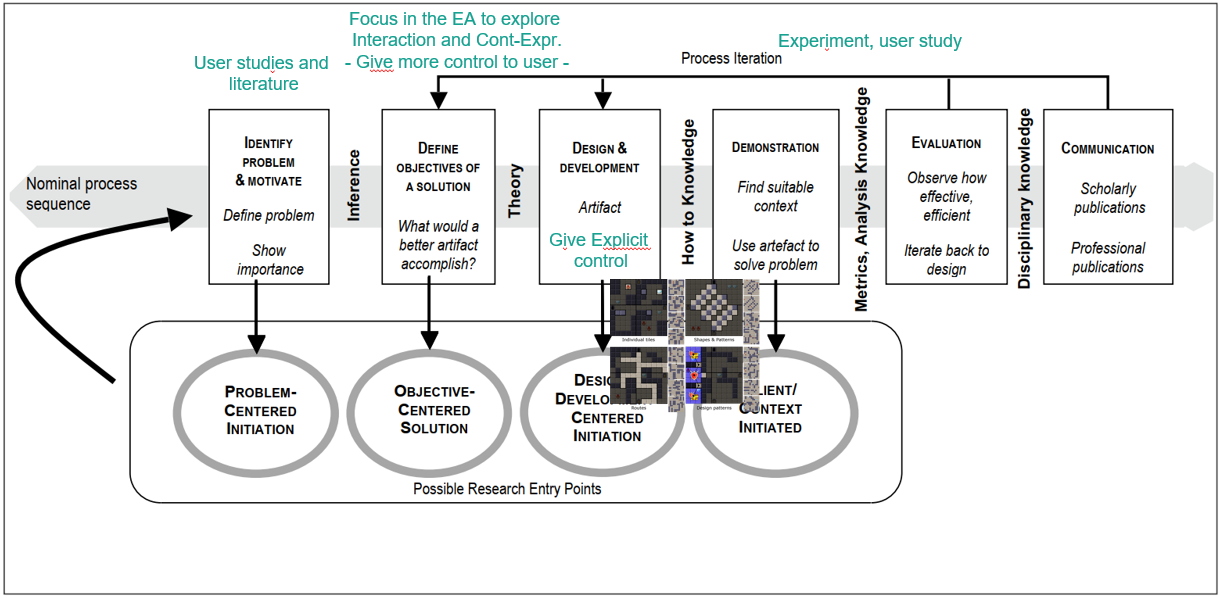
\includegraphics[width=\textwidth]{figures/Methodology-figs/lockingtiles-dsrm.png}
% \caption{DSRM cycle of the first study~\cite{Alvarez2018a}} \label{figs:lockingTiles}
% \end{figure}

% Figure~\ref{figs:lockingTiles} shows the first DSRM process seeking the development, exploration, and evaluation of providing direct control over multiple steps in the EA i.e. crossover and mutation, through locking tiles that needed to be preserved~\cite{Alvarez2018a}. For this process, two iterations were performed, one to evaluate the artifact through simulations to study to what extent the approach was controlling the evolutionary process. The second iteration focused on evaluating the approach's usability and assessing how designers interacted with the systems and responded to the suggestions. The solutions were deemed positive, but the expressivity of the algorithm was affected, and the workload of designers increased to some extent, given that they needed to provide what was to be preserved.

% \begin{figure}
% 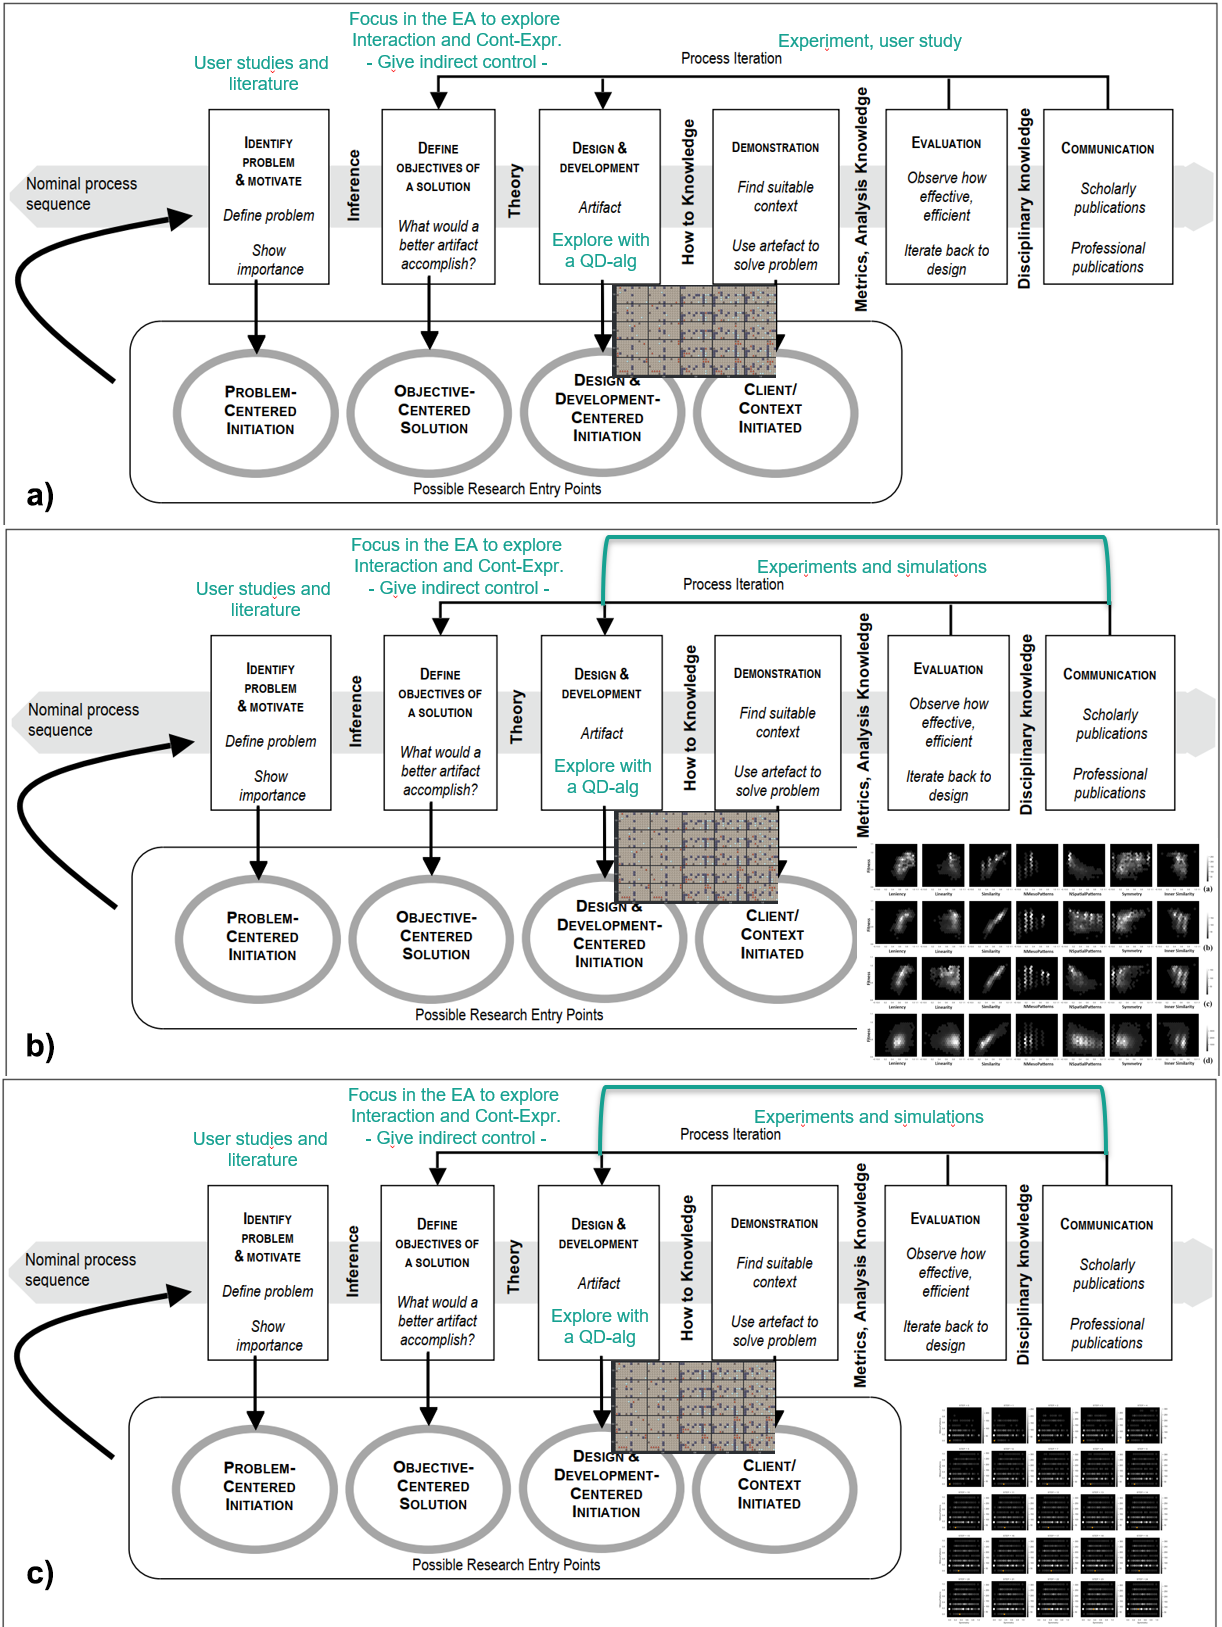
\includegraphics[width=\textwidth]{figures/Methodology-figs/ICMAPE-dsrm.png}
% \caption{DSRM cycle of the second study~\cite{alvarez2019empowering}. a) denotes the first and second iteration~\cite{alvarez2019empowering}, b) the third iteration where the evaluation was on static levels~\cite{Alvarez2020-ICMAPE}, and c) the fourth and current iteration where IC MAP-Elites was evaluated in a dynamic environment~\cite{Alvarez2020-ICMAPE-interactive}.} \label{figs:icmape}
% \end{figure}

% Moreover, informed by the user study evaluating the tool and it is new features and underlying-AIs~\cite{Alvarez2018}, a new DSRM process was started. In figure~\ref{figs:icmape}, it is shown this parallel cycle within the same objective, exploring interaction with the EA. The focus of this process was to study how to use Quality-Diversity (QD) algorithms to balance controllability and expressivity due to the special properties of these algorithms, where the focus is on searching a substantial area of the solution space while yielding high-performing individuals~\cite{gravina2019procedural,Pugh2016}. Therefore, the development was set into producing a variant of a recent and popular QD algorithm called MAP-Elites~\cite{Mouret2015}. The proposed approach named Interactive Constrained MAP-Elites (IC MAP-Elites)~\cite{Alvarez2020-ICMAPE}, is a variant of the Constrained MAP-Elites, introduced by Khalifa et al.~\cite{Khalifa2018}, combined with Interactive Evolution.

% The algorithm yielded very positive results, and have had most of the focus in this thesis. The process is still on-going, and four iterations have been done. The first (fig. ~\ref{figs:icmape}.a), when the algorithm was proposed~\cite{alvarez2019empowering}, evaluated through simulations the properties of QD algorithms, and the possibilities it brings. The second iteration focused on evaluating IC MAP-Elites through controlled experiments with an informal user study. Designers were asked to try the tool without special focus in the QD algorithm, but rather as a more general test. The results from such a study informed the next DSRM process focused on modeling designers. Moreover, the third and fourth iterations (fig. ~\ref{figs:icmape}.b and .c, respectively), focused on a dynamic evaluation of IC MAP-Elites to identify and explore the generative space of the algorithm and its properties and dynamics in both, a static scenario using all pair of dimensions~\cite{Alvarez2020-ICMAPE}, and dynamic one following simulations of the MI-CC interactive loop~\cite{Alvarez2020-ICMAPE-interactive}.
% %This process is still on-going, and two iterations have been done—the first when the algorithm was proposed.

% \subsubsection{Focus in moving towards designer modeling through different adaptive models.} While the previous DSRM cycle is not over yet, conducting those studies pointed out key directions to focus and new aims to address the above-mentioned RQs. The objective with the following cycles is to explore ways towards designer modeling. This in order to reduce the designer's fatigue and create better and adaptive experiences that take into consideration an individual's preferences, styles, and in general, their design and creative process.

% \begin{figure}
% 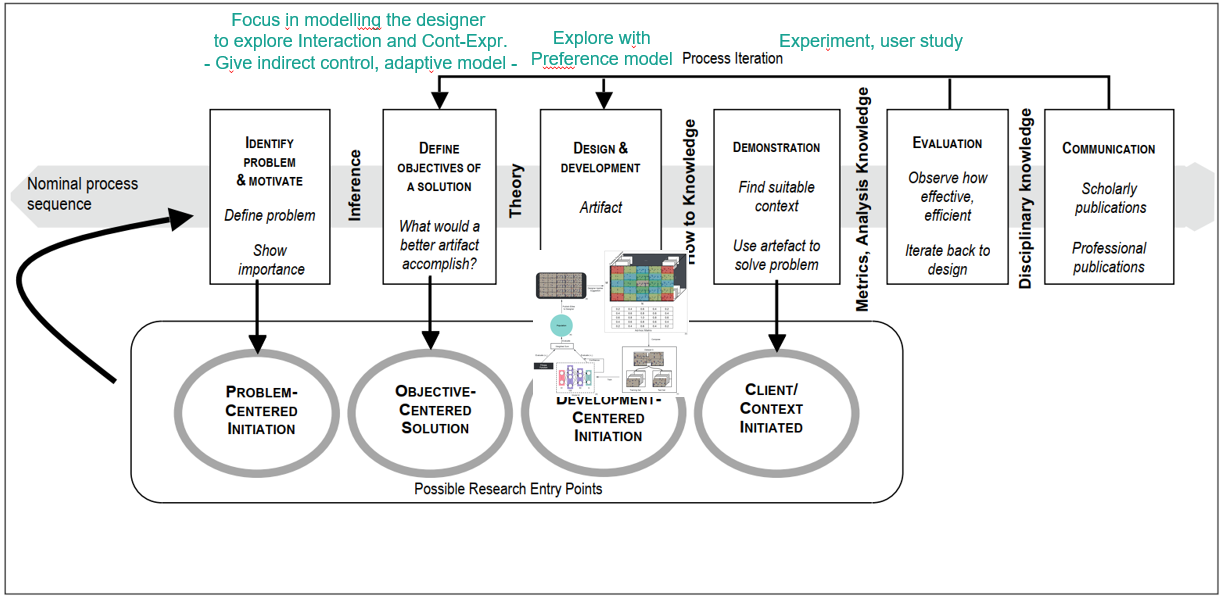
\includegraphics[width=\textwidth]{figures/Methodology-figs/desPref-dsrm.png}
% \caption{DSRM cycle of the third study~\cite{Alvarez2020-DesignerPreference}.} \label{figs:desPrefDSRM}
% \end{figure}

% \begin{figure}
% 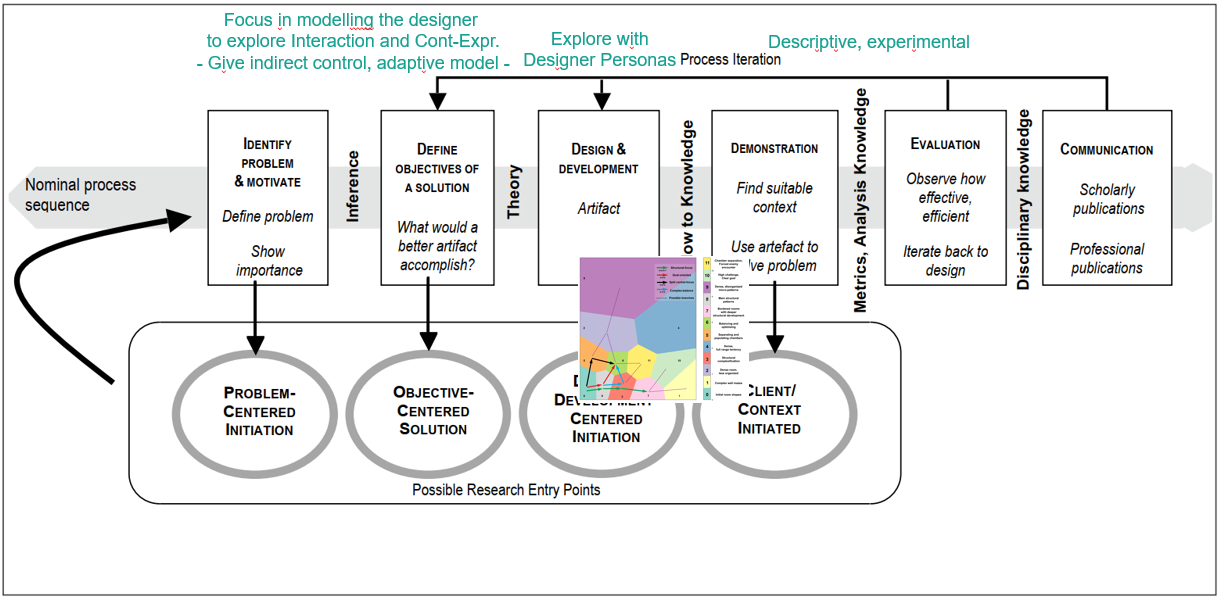
\includegraphics[width=\textwidth]{figures/Methodology-figs/desPersonas-dsrm.png}
% \caption{DSRM cycle of the fourth study~\cite{alvarez2020-designerpersonas}.} \label{figs:desPersDSRM}
% \end{figure}

% Figure~\ref{figs:desPrefDSRM} presents the first cycle towards designer modeling by exploring the usage of a preference model~\cite{Alvarez2020-DesignerPreference}. In this model informed by the findings in ~\cite{alvarez2019empowering,Alvarez2018}, and the unpublished user study of the IC MAP-Elites, the focus was on automatically modeling the preferences of the designer. This was done by collecting new data as the designer was applying suggestions by the EA, and training a neural network (ANN) with the distribution of the provided suggestions. Figure~\ref{figs:desPrefModel} exemplify the procedure. Furthermore, the preference model went through two iterations, the first, where the model i.e. ANN, was evaluated to explore the accuracy and usability, and a second, where the model was tested in practice by beginner designers.

% Moreover, figure~\ref{figs:desPersDSRM} presents another cycle within the frame of adaptive models. In this case, the focus was on dividing the design space to form clusters of room styles based on the data collected from previous user studies. Analyzing the designer's edition steps when using the tool in relation to the new clusters, the study identified four archetypical paths taken by most designers, named Designer Personas~\cite{alvarez2020-designerpersonas}. The contribution was evaluated through descriptive methods because while data was used to form the Designer Personas, its usability and support are informed by literature.

\subsection{Methodology Discussion}

This thesis embraces~\acrshort{dsrm} as the principal methodology employed to explore, analyze, and address the different artifacts and RQs. However, it is essential to have a methodology discussion for those methodologies that could have been as valid in the frame of this thesis, with their own set of tradeoffs. 

%Before moving towards the different evaluation methods followed so far and that I have identified as necessary to address my RQs, I would like to bring the attention to other methodologies that could be as valid as well in the frame of this thesis. 

The field of Human-Computer Interaction (HCI) has studied for a long time the ways interactions can be created, approached, and established to foster, encourage, and address different functionalities and capabilities of humans. Likewise, the interaction between humans and AI has been the focus of much of the recent work by the community, which is now developing further than the computer science and information system frontiers towards intertwining with many other science fields~\cite{rahwan_machine_2019}. 

However, these interactions, especially when the human and the AI do not necessarily need to have asymmetric functionalities (i.e., having an intelligent system that merely assist) and that both can participate in reciprocal stimuli to reach a common goal, still have uncountable challenges and questions to research and explore. This is thus, one of the motivations behind this thesis, which in part calls for the use of a more exploratory and holistic methodology that can then observe, analyze, model, and address the unknown space of problems and solutions.

An exploratory methodology that could have been used is~\acrfull{rtd}~\cite{rtd-zimmerman2007} since, after all, the iterative design of multiple artifacts and the investigation of how this open new spaces in the research is important to understand those unknown spaces.~\acrshort{rtd} is a methodology from the field of~\acrshort{hci}, which aims at tackling ``Wicked Problems’’ meaning unexplored, unclear, and complex scenarios and situations that are not easily simplified.~\emph{Design Thinking} is the design process used to describe~\acrshort{rtd}, consisting of \emph{grounding, ideation, and iteration}. Following the~\acrshort{rtd} methodology, one addresses these problems through a holistic approach with an iterative process that reframes the problem through designing artifacts and prototypes as a means of knowledge. The knowledge generated from these prototypes reframes the space of problems and solutions, which in turn provides an important opportunity for researchers on focusing in the future state and on defining a preferred state to be achieved~\cite{rtd-critique-zimmerman2010}. 

Moreover,~\acrfull{pd} matches as well the requirements of this thesis, especially understanding that the research while focusing on the development of technological innovations and artifacts, has a human-centered perspective~\cite{ParticipatoryDesign-Spinuzzi2005}.~\acrshort{pd} is a methodology that involves the target user of a specific type of design in the design and research process. Through this, the necessities of the target user are gathered, and their visions, expertise, and understanding are incorporated and included in the proposed solutions. Usually, the researcher wants to explore certain aspects of an unknown space, although it is not necessary to be unknown, together with the target users. These users understand and manage different problems and solutions in the design space, thus by co-designing the solution, they are involved and are part of the solution rather than this being delivered to them~\cite{ParticipatoryDesign-Spinuzzi2005}. 

%I need to check a bit more this methodology. Furthermore, Björgvinsson et al \cite{bjorgvinsson-democratizing-innovation} coined the term ``democratizing innovation’’ to further connect participatory design results  the 

These methodologies could allow the work to be, in principle, more exploratory and letting the users actually participate in the design of the human-AI interaction loop. However, through the methods within~\acrshort{dsrm} and the research plan, this thesis has explored to a certain extent the incorporation of important aspects of these methodologies. While the main focus is on~\acrshort{edd} to explore this interaction; throughout this thesis, multiple prototypes and artifacts addressing the underlying AI have been developed to explore different design capabilities and interactions that have helped reframed problems and space of solutions, akin to~\acrshort{rtd}.

Furthermore, we have managed to evaluate qualitative aspects of the tools and the interaction designers have with it through user studies. Thus, from our focus groups (i.e., game designers), there are important points to approach and address that motivates the next steps in the thesis. For instance, in the user study done in~\textsc{paper i}, it was a recurrent topic that designers wanted more control over the tool and algorithms. Designers did not see a relation between their work and what the tool offered (i.e., preserving their design, intentions, and ideas), while of course, still expecting interesting solutions from the algorithm. This topic, supported by previous research, have chained a set of improvements and implementations in order to balance the requirements from designers. For instance, in~\textsc{papers iv, ix}, and in general, the steps towards capturing and developing designer models to be used as a complement evaluation in the interaction between the designer and the artificial design, have been motivated by the struggle and balance between controllability and expressivity.  

% \begin{figure}
% 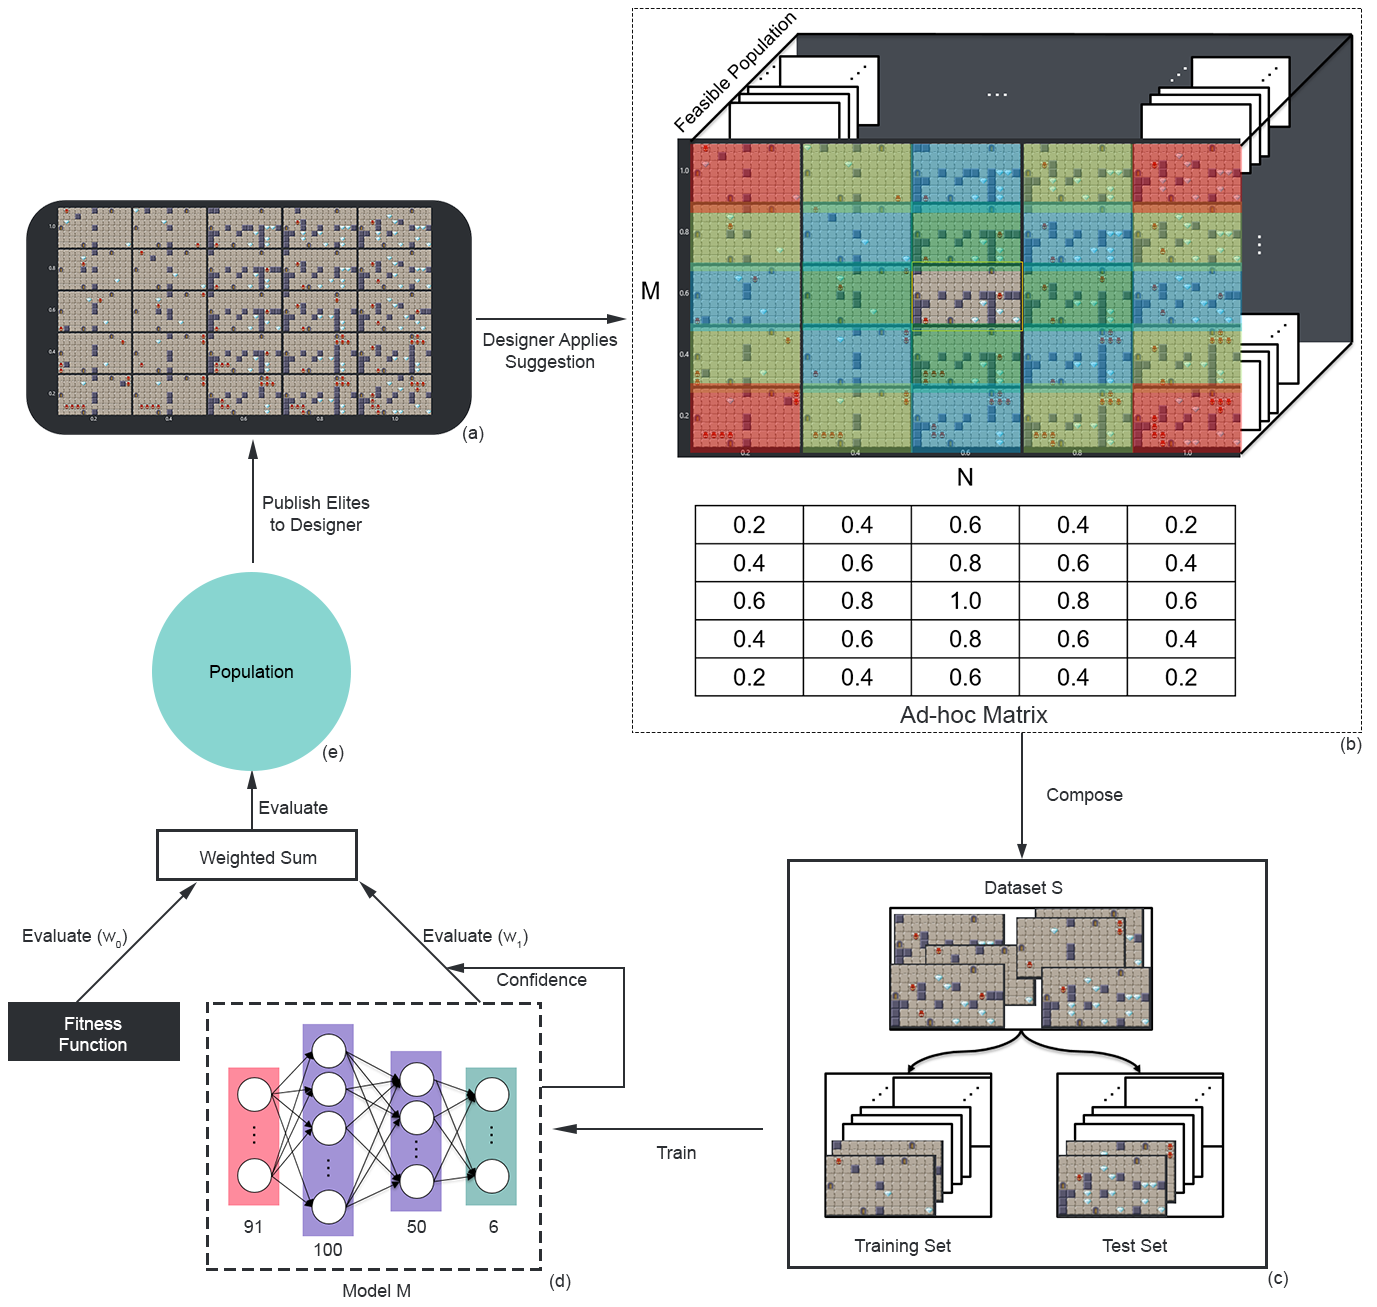
\includegraphics[width=\textwidth]{figures/fig4.png}
% \caption{Overview of the Designer Preference Model integrated into the fitness function of EDD. Elites are published and shown to the designer in a grid fashion (a), and once the designer chooses and applies one of the suggestions, an ad-hoc matrix is created based on the position of the selected suggestion to estimate the preference of suggestions (b). The ad-hoc matrix is then applied to all the elites in the grid, and the feasible populations within the EA cells to compose a general dataset $S$ with rooms labeled by the estimated preference. The composed dataset $S$ is then subdivided into a training set (90\%) and test set (10\%), both with the same label distribution (c). The dataset is used to train a model $M$, which is a relatively small neural network, for 20 epochs (d). The  model is then used to evaluate the population of the EA together with the current fitness function in a weighted sum, with the weight of the model $M$ conditioned by the confidence of the network (e).} \label{figs:desPrefModel}
% \end{figure}



